% \begin{wrapfigure}{!r}{0.45\textwidth}
%     \centering
%     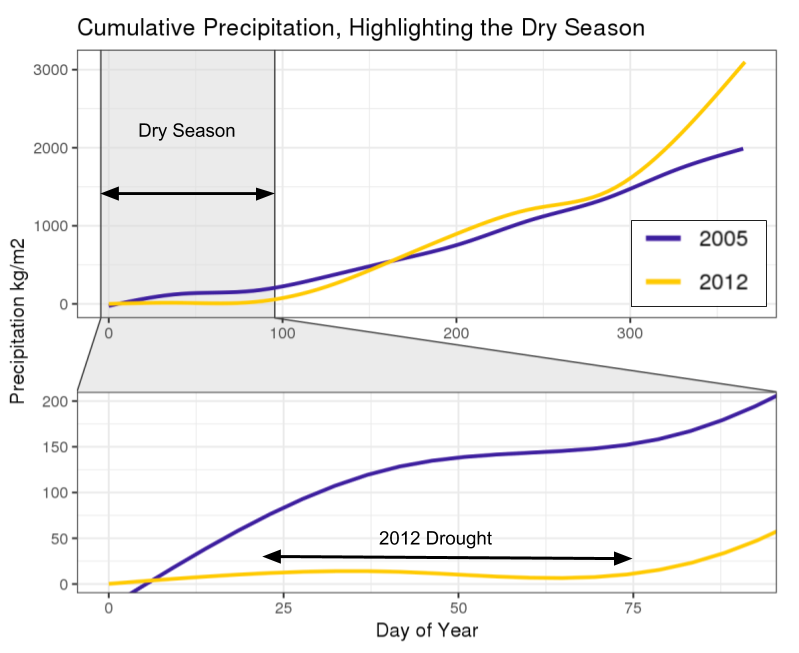
\includegraphics[width=.45\textwidth]{Hydro_Paper_LaTeX/Hydro_Paper_Figures/precip.png}
%     \caption[Precipitation]{Precipitation: To be more informative, this plot should also have the average of all the available years to get a better idea of how "extreme" these two scenarios actually are.}
%     \todoa{caption}
%     \label{fig:precip}
% \end{wrapfigure}

\begin{figure}[!h]
    \centering
    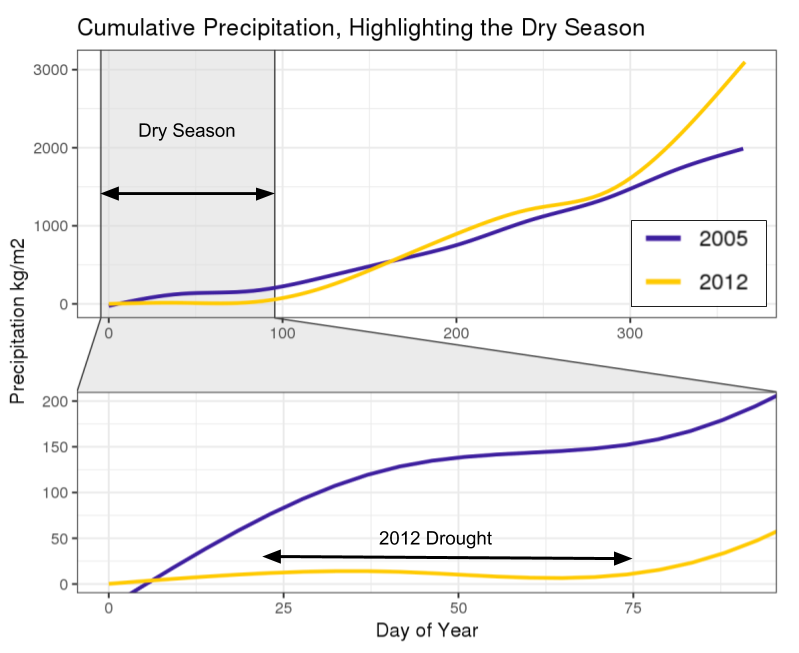
\includegraphics[width=.65\textwidth]{Hydro_Paper_LaTeX/Hydro_Paper_Figures/precip.png}
    \caption[Precipitation]{Cumulative precipitation at Barro Colorado Island, Panama for the years 2012 (yellow) and 2005 (purple). The pictured years have the most divergent climactic conditions over the dry season, with 2012 having an dry and prolonged dry season and 2005 having a short and wet dry season. 
    \todoq{To be more informative, this plot should also have the average of all the available years to get a better idea of how "extreme" these two scenarios actually are.}}
    % \todoa{caption}
    \label{fig:precip}
\end{figure}
